
%----------------------------------------------------------------------------------------
%	PACKAGES AND OTHER DOCUMENT CONFIGURATIONS
%----------------------------------------------------------------------------------------


\documentclass[
11pt, % The default document font size, options: 10pt, 11pt, 12pt
%oneside, % Two side (alternating margins) for binding by default, uncomment to switch to one side
english, % ngerman for German
singlespacing, % Single line spacing, alternatives: onehalfspacing or doublespacing
%draft, % Uncomment to enable draft mode (no pictures, no links, overfull hboxes indicated)
%nolistspacing, % If the document is onehalfspacing or doublespacing, uncomment this to set spacing in lists to single
%liststotoc, % Uncomment to add the list of figures/tables/etc to the table of contents
%toctotoc, % Uncomment to add the main table of contents to the table of contents
%parskip, % Uncomment to add space between paragraphs
%nohyperref, % Uncomment to not load the hyperref package
headsepline, % Uncomment to get a line under the header
%chapterinoneline, % Uncomment to place the chapter title next to the number on one line
%consistentlayout, % Uncomment to change the layout of the declaration, abstract and acknowledgements pages to match the default layout
]{MastersDoctoralThesis} % The class file specifying the document structure

\usepackage[utf8]{inputenc} % Required for inputting international characters
\usepackage[T1]{fontenc} % Output font encoding for international characters

\usepackage{palatino} % Use the Palatino font by default

\usepackage[backend=bibtex,style=authoryear,natbib=true]{biblatex} % Use the bibtex backend with the authoryear citation style (which resembles APA)
\addbibresource{references.bib} % The filename of the bibliography

\usepackage[autostyle=true]{csquotes} % Required to generate language-dependent quotes in the bibliography

\usepackage{amsmath}
\usepackage{graphicx}
\usepackage{pdfpages}
\usepackage{csvsimple}
\usepackage{cleveref}
\usepackage{booktabs}

%----------------------------------------------------------------------------------------
%	MARGIN SETTINGS
%----------------------------------------------------------------------------------------

\geometry{
	paper=a4paper, % Change to letterpaper for US letter
	inner=2.5cm, % Inner margin
	outer=3.8cm, % Outer margin
	bindingoffset=.5cm, % Binding offset
	top=1.5cm, % Top margin
	bottom=1.5cm, % Bottom margin
	%showframe, % Uncomment to show how the type block is set on the page
}

%----------------------------------------------------------------------------------------
%	THESIS INFORMATION
%----------------------------------------------------------------------------------------

\thesistitle{Extracting Knowledge from Complex Networks} % 
\supervisor{Dr. Shan \textsc{He}} 
\examiner{} 
\degree{Doctor of Philosophy}
\author{David \textsc{McDonald}} 
\addresses{} 

\subject{Computer Science} 
\keywords{Complex networks} 
\university{\href{www.bham.ac.uk}{University of Birmingham}}
\department{\href{www.cs.bham.ac.uk}{Department of Computer Science}} 
%\group{\href{http://researchgroup.university.com}{Research Group Name}} % Your research group's name and URL, this is used in the title page, print it elsewhere with \groupname
\faculty{\href{www.cs.bham.ac.uk}{Computer Science}} 

\AtBeginDocument{
\hypersetup{pdftitle=\ttitle} % Set the PDF's title to your title
\hypersetup{pdfauthor=\authorname} % Set the PDF's author to your name
\hypersetup{pdfkeywords=\keywordnames} % Set the PDF's keywords to your keywords
}

\begin{document}

\frontmatter % Use roman page numbering style (i, ii, iii, iv...) for the pre-content pages

\pagestyle{plain} % Default to the plain heading style until the thesis style is called for the body content

%----------------------------------------------------------------------------------------
%	TITLE PAGE
%----------------------------------------------------------------------------------------

\begin{titlepage}
\begin{center}

\vspace*{.06\textheight}
{\scshape\LARGE \univname\par}\vspace{1.5cm} % University name
\textsc{\Large Doctoral Thesis Proposal}\\[0.5cm] % Thesis type

\HRule \\[0.4cm] % Horizontal line
{\huge \bfseries \ttitle\par}\vspace{0.4cm} % Thesis title
\HRule \\[1.5cm] % Horizontal line
 
\begin{minipage}[t]{0.4\textwidth}
\begin{flushleft} \large
\emph{Author:}\\
\href{dxm237@cs.bham.ac.uk}{\authorname} 
\end{flushleft}
\end{minipage}
\begin{minipage}[t]{0.4\textwidth}
\begin{flushright} \large
\emph{Supervisor:} \\
\href{s.he@cs.bham.ac.uk}{\supname} 
\end{flushright}
\end{minipage}\\[3cm]
 
\vfill

\large \textit{A thesis proposal submitted in fulfilment of the requirements\\ for the degree of \degreename}\\[0.3cm] % University requirement text
\textit{in the}\\[0.4cm]
\deptname\\[2cm] % Research group name and department name
 
\vfill

{\large \today}\\[4cm] % Date
%\includegraphics{Logo} % University/department logo - uncomment to place it
 
\vfill
\end{center}
\end{titlepage}

%----------------------------------------------------------------------------------------
%	DECLARATION PAGE
%----------------------------------------------------------------------------------------

%\begin{declaration}
%\addchaptertocentry{\authorshipname} % Add the declaration to the table of contents
%\noindent I, \authorname, declare that this thesis titled, \enquote{\ttitle} and the work presented in it are my own. I confirm that:
%
%\begin{itemize} 
%\item This work was done wholly or mainly while in candidature for a research degree at this University.
%\item Where any part of this thesis has previously been submitted for a degree or any other qualification at this University or any other institution, this has been clearly stated.
%\item Where I have consulted the published work of others, this is always clearly attributed.
%\item Where I have quoted from the work of others, the source is always given. With the exception of such quotations, this thesis is entirely my own work.
%\item I have acknowledged all main sources of help.
%\item Where the thesis is based on work done by myself jointly with others, I have made clear exactly what was done by others and what I have contributed myself.\\
%\end{itemize}
% 
%\noindent Signed:\\
%\rule[0.5em]{25em}{0.5pt} % This prints a line for the signature
% 
%\noindent Date:\\
%\rule[0.5em]{25em}{0.5pt} % This prints a line to write the date
%\end{declaration}

%\cleardoublepage

%----------------------------------------------------------------------------------------
%	QUOTATION PAGE
%----------------------------------------------------------------------------------------

\vspace*{0.2\textheight}

\noindent\enquote{\itshape I'm fascinated by the idea that genetics is digital. A gene is a long sequence of coded letters, like computer information. Modern biology is becoming very much a branch of information technology.}\bigbreak

\hfill Richard Dawkins

%----------------------------------------------------------------------------------------
%	ABSTRACT PAGE
%----------------------------------------------------------------------------------------

\begin{abstract}
\addchaptertocentry{\abstractname} % Add the abstract to the table of contents
Throughout nature, we observe complex systems everywhere -- from the social interactions of individuals within society, right down to the interrelation and cooperation of proteins, genes and metabolites within the cell. When modelling these systems, sometimes it is convenient to represent them as networks of different entities and relationships. So the problem of understanding these systems is the problem of building sufficiently powerful network models and devising methodologies to extract useful features from them. This thesis proposal will focus upon these challenges within the context of computational biology -- namely, how can we make best sense of the vast amounts of data produced in the post-genome age? We propose novel information extraction techniques from multilayer networks -- representing the intercellular world -- in the form of network embedding and module identification techniques. These models will provide an insight into the formation of these complex systems and help to guide bioscientists by offering real, testable hypotheses in the form of new interaction and functional predictions. 
\end{abstract}

%----------------------------------------------------------------------------------------
%	ACKNOWLEDGEMENTS
%----------------------------------------------------------------------------------------

%\begin{acknowledgements}
%\addchaptertocentry{\acknowledgementname} % Add the acknowledgements to the table of contents
%The acknowledgments and the people to thank go here, don't forget to include your project advisor\ldots
%\end{acknowledgements}

%----------------------------------------------------------------------------------------
%	LIST OF CONTENTS/FIGURES/TABLES PAGES
%----------------------------------------------------------------------------------------

\tableofcontents % Prints the main table of contents

\listoffigures % Prints the list of figures

%\listoftables % Prints the list of tables

%----------------------------------------------------------------------------------------
%	ABBREVIATIONS
%----------------------------------------------------------------------------------------

%\begin{abbreviations}{ll} % Include a list of abbreviations (a table of two columns)
%
%\textbf{LAH} & \textbf{L}ist \textbf{A}bbreviations \textbf{H}ere\\
%\textbf{WSF} & \textbf{W}hat (it) \textbf{S}tands \textbf{F}or\\
%
%\end{abbreviations}

%----------------------------------------------------------------------------------------
%	PHYSICAL CONSTANTS/OTHER DEFINITIONS
%----------------------------------------------------------------------------------------

%\begin{constants}{lr@{${}={}$}l} % The list of physical constants is a three column table
%
%% The \SI{}{} command is provided by the siunitx package, see its documentation for instructions on how to use it
%
%Speed of Light & $c_{0}$ & \SI{2.99792458e8}{\meter\per\second} (exact)\\
%%Constant Name & $Symbol$ & $Constant Value$ with units\\
%
%\end{constants}

%----------------------------------------------------------------------------------------
%	SYMBOLS
%----------------------------------------------------------------------------------------

%\begin{symbols}{lll} % Include a list of Symbols (a three column table)
%
%$a$ & distance & \si{\meter} \\
%$P$ & power & \si{\watt} (\si{\joule\per\second}) \\
%%Symbol & Name & Unit \\
%
%\addlinespace % Gap to separate the Roman symbols from the Greek
%
%$\omega$ & angular frequency & \si{\radian} \\
%
%\end{symbols}

%----------------------------------------------------------------------------------------
%	DEDICATION
%----------------------------------------------------------------------------------------

%\dedicatory{For/Dedicated to/To my\ldots} 

%----------------------------------------------------------------------------------------
%	THESIS CONTENT - CHAPTERS
%----------------------------------------------------------------------------------------

\mainmatter % Begin numeric (1,2,3...) page numbering

\pagestyle{thesis} % Return the page headers back to the "thesis" style

%\include{Chapters/Chapter1}
%\include{Chapters/Chapter2} 
%\include{Chapters/Chapter3}
%\include{Chapters/Chapter4} 
%\include{Chapters/Chapter5} 

\chapter{Introduction}



Most complex systems observed in nature can be represented as a complex network. A complex network is a highly heterogeneous object that is represented as a mathematical graph that is comprised of non-trivial and non-uniform features. 


%	While the early belief was that the interactions of such seemingly unrelated things as proteins, social interactions and the internet were random and unconnected, it has since been shown that, surprisingly, most real world systems have share a lot of similarities -- a revelation that gripped the scientific community and is the reason for the their continuing popularity in the literature across many diverse areas of study. Areas such as computer science, medicine and social analyses.

Despite being characterised as complex objects, we have observed that many real world networks, from protein interaction networks, to the internet, possess shared features that unite such seemingly disparate subject and give rise to the prevailing popularity of their study. For example, we have observed that these complex networks follow scale-free distribution of node degree (often with exponent $\gamma\in [2, 3]$) (\cite{barabasi1999emergence,barabasi2009scale}). Connections are preferentially made between nodes with a probability proportional to their existing degree, giving rise to the so-called preferential attachment model, a model that adheres to the old `popularity is attractive' adage. Furthermore, complex networks also are characterised by the `small world' phenomenon, where one would expect a small average shortest path length and a high degree of clustering (\cite{watts1998collective}); and are typically very sparse with the number of edges in the same order as the number of nodes. 

The work proposed here will focussed primarily upon the study of complex networks within the context of computational biology. Given the explosion of data available to us thanks to modern experimentation techniques, the need for modelling such data, has never been greater. Through the medium of complex networks, researchers wish to simplify and represent the raw data in a data-driven and scientifically justified way, such that is becomes useful for the purposes of making functional predictions and tracing the causes of observed disease phenotypes. 

Already, we have seen the application of complex network models to the problems of identification of biologically relevant modules according to genetic expression profiles (\cite{ideker2002discovering}); the multi scale detection of the function and structure of brain networks (\cite{ashourvan2017multi}); and testable protein functional predictions (\cite{palla2005uncovering,zhang2016integrated}). And with the growing availability of data and drive of the network science community, models are becoming more and more complex, with the integration of multiple types of data and more sophisticated analysis techniques. It is the hope of the work proposed here to further this burgeoning field by proposing novel, integrative network models that allow for the extraction of testable hypotheses based on the data currently available to us.


%\chapter{Thesis Statement}
%
%The work proposed in this document shall...
%
%\section{Research questions}
%
%The following research questions have been selected to facilitate such an investigation:
%
%\begin{enumerate}
%	\item Can a multi-layer network model be constructed such that the hyperbolic metric space that underpins complex network formation be uncovered for multi-layer networks?
%	\item What interpretable information, such as disease modules or functional predictions, can be extracted from such a model?
%	\item My constructing data-driven models, can we predict protein abundance and phosphorylation?
%\end{enumerate}
%
%
%\section{Significance}
%?




\chapter{Literature Review}
Network science is the interdisciplinary endeavour of making sense of the complex networks that we observe in nature. It unites scientists from such varied fields as mathematics, computer science, medicine, biology and sociology. Researchers from all these fields and more have contributed their expertise and perspective. This section aims to give a brief overview of some of the interesting areas of research happening in this field. For the purpose of brevity, the review presented here will only focus on the fundamental concepts that will prove to be relevant in the work proposed here. For a more general overview of network science, the reader is pointed towards \cite{barabasi2002linked}, a book written by Albert-L{\'a}szl{\'o} Barab{\'a}si, a well respected and prolific figure in this field.

\section{Community Detection}

Many real-world networks contain subsets of nodes that contain a higher degree of inter-connectivity than the rest of the network
(\cite{girvan2002community,palla2005uncovering,lancichinetti2009detecting}).
These subsets are commonly referred to as communities. 
A rigorous definition for a `community' within a network still seems to elude the scientific community( \cite{lancichinetti2009detecting}).
However, the most popular definition among scholars is the planted l-partition model.
This was popularised thanks to Girvan and Newman in their seminal work \cite{girvan2002community} and states that as long the probability of a node being connected to its group is greater than the probability of it being connected to the rest of the graph, then those groups are communities. 
`Community detection' is the name given to the problem of finding the underlying community structure in a given network (\cite{girvan2002community}). 
For example, groups of friends in a social network, functional modules in Protein-Protein Interaction (PPI) networks and scientific disciplines in co-authorship networks.

%	Most real world networks do not solely contain communities at one scale \cite{lancichinetti2009detecting,yang2013hierarchical}. 
%	They contain super communities that may contain sub-communities, that may, in turn, contain their own sub communities.
%	And so on. 
%	Delving deeper into the community structure may offer some insight into how these processes work.
%	For example, hierarchical analysis of protein-protein interaction networks may help to identify subsets of functionally-related proteins that interact together strongly within an established community representing some biological process.

But, a general community detection algorithm does not yet exist.
Many existing algorithms suffer from a number of issues. 
To name a few:
The number and scale of communities must be known a-priori, which in most real applications, is infeasible.
Additionally, the relationships between communities, both one the same level and at different ones, is lost.
Identifying not only the community itself, but its position in the network as a whole, provides further insight into the often abstract interactions that comprise complex networks and so preserving this information when analysing a network is paramount.
And, in some cases, the algorithms cannot deal with special cases: for example, modularity-based methods suffer from the so-called `resolution limit' (\cite{fortunato2007resolution}).

\begin{figure}
	\centering
	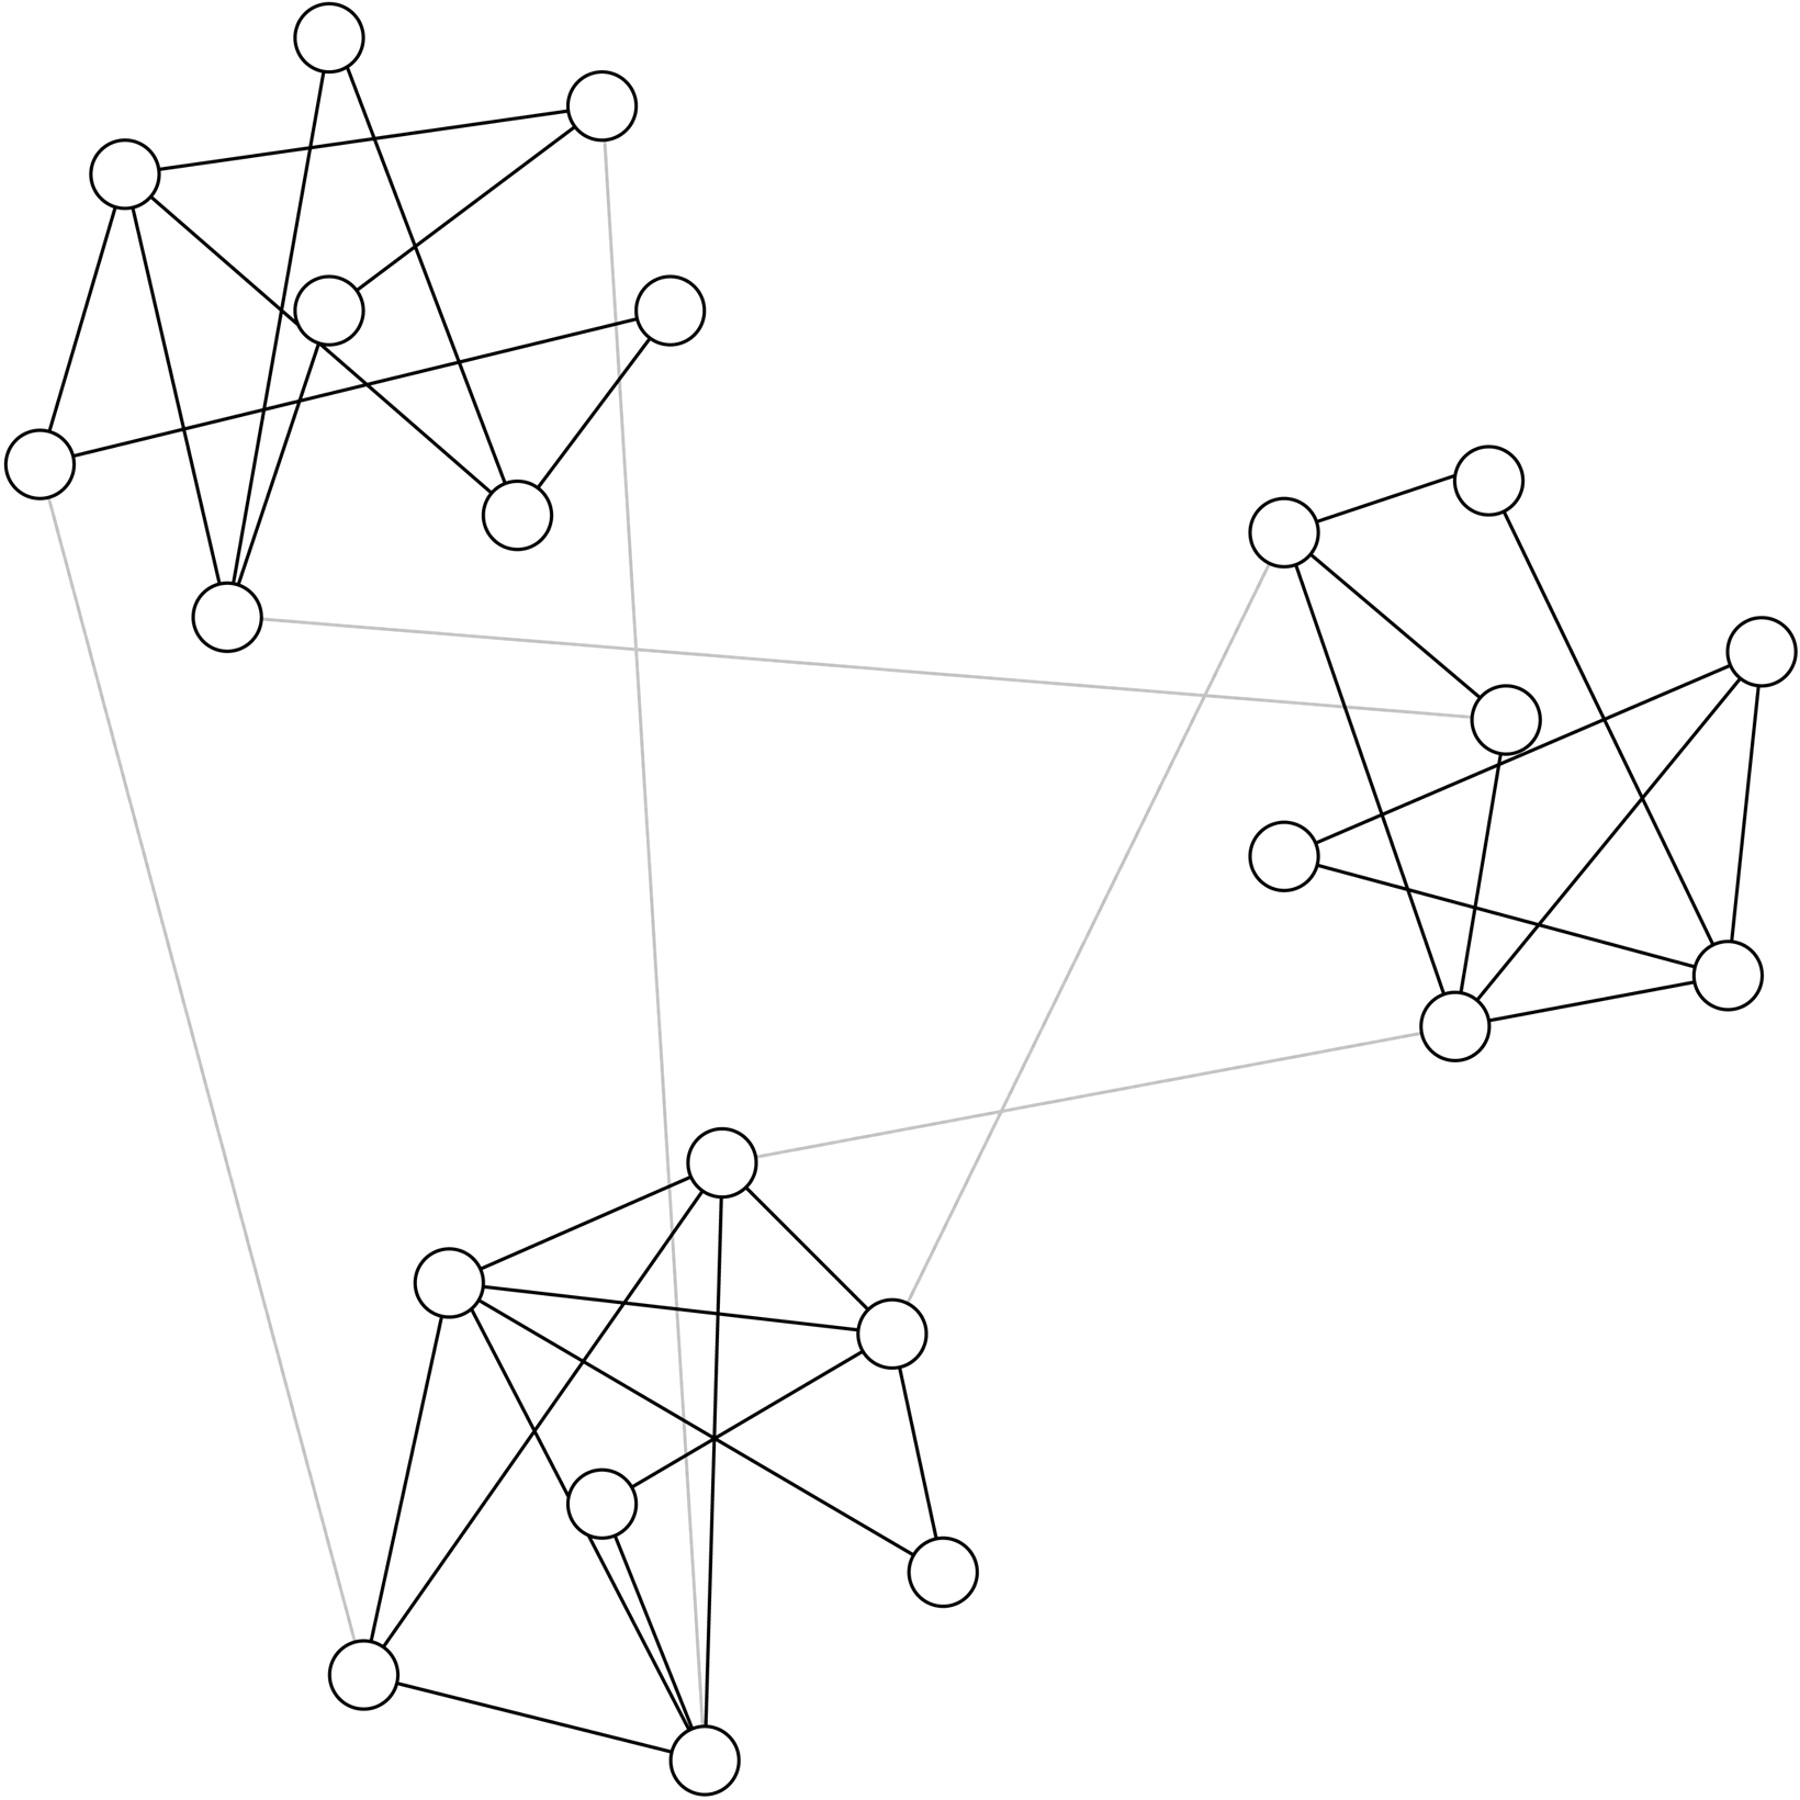
\includegraphics[width=\textwidth]{figures/communities}
	\caption[Communities in a network]{Representation of a network with three communities. The network has a higher proportion of edges between nodes of the same community than edges between nodes in different communities. Figure taken from \cite{girvan2002community}.}
\end{figure}

\subsection{Cut-Based and Spectral Approaches}
The flagship Kernighan-Lin algorithm  (\cite{kernighan1970efficient}) focused on `cutting' the network into modules, in such a way that the number of edges cut was minimized. 
However, this often favoured cuts of small, peripheral subgraphs, so it was adapted into ratio cut (\cite{wei1991ratio}), normalised cut (\cite{shi2000normalized}) and min-max cut (\cite{ding2001min}) that took the number of nodes in each resulting sub-graph into account, and thus resulted in a partition that was more balanced.

Contemporary cut-based approaches are concerned more with edges, rather than vertices and gave rise to a new measure for a good cut, called conductance.
%\begin{align}
%\phi(S) = \frac{c_s}{\min(Vol(S),Vol(V \setminus S)} 
%\end{align}
%with
%\begin{align}
%c_s = |\{(u,v) : u \in S, v \not\in S\}|
%\end{align}
Conductance is still prolific in the literature: it has been used to detect communities in bipartite networks (\cite{barber2007modularity}), combined with PageRank (\cite{andersen2006local}) and used as the basis for a greedy optimisation algorithm (\cite{lancichinetti2009community}) capable of finding overlapping communities at different scales. 

Spectral clustering dates back to the work of Donath and Hoffman in 1973 (\cite{donath1973lower}). 
However, it was popularized in the early 2000s (\cite{shi2000normalized,ng2002spectral,ding2004tutorial}). 
Spectral methods rely upon constructing Laplacian matrices from the raw network data and eigen-decomposing them. 
Clustering the resulting eigenvectors results in clusters of the original data points. 
Spectral approaches have many advantages over other techniques and, as a result, they have become popular in the machine learning community for clustering  on non-linear manifolds. 
According to \cite{von2007tutorial}, `these methods do not make assumptions about the form of the clusters' and are capable of correctly identifying typically challenging clusters, such as the famous two spirals example. 
For community detection, they have the additional benefit of efficiency, especially if the graph adjacency matrix is sparse. 


\subsection{Modularity-Based Approaches}
The seminal work of Girvan and Newman (\cite{girvan2002community}) marked a significant advance in the field by providing the first quantitative measure of a community: modularity. 
The modularity of a partition of a network 
defined as
\begin{align} 
\label{modularity}
Q = \sum_{s=1}^m \bigg[ \frac{l_s}{L} - \bigg( \frac{d_s}{2L} \bigg)^2\bigg]
\end{align}
scores a network partition by comparing the number of links inside a given module with the expected number that would be found in a random graph of the same size and degree sequence. 
Here, $m$ is the number of modules in the partition, $l_s$ is the number of links in module $s$, $L$ is the total number of links in the network and $d_s$ is the total degree of the nodes in $s$. 
%The first term in equation \ref{modularity} is the fraction of links inside $s$ and the second term represents the expected fraction of random links in the graphs to be in the module. 
Girvan and Newman propose a hierarchical divisive algorithm that removes edges based on their `betweenness' (the number of shortest paths from two nodes in the network that go through them) until the modularity quality function is maximized. 
The early work of Girvan and Newman has since been expanded upon.
For example, edge clustering in favour of edge-betweenness (\cite{radicchi2004defining}), iteratively adding links to a module based on their expected increase in modularity (\cite{clauset2004finding}), and multi-stage local optimization in the popular Louvain algorithm (\cite{blondel2008fast}).

%Radicchi at al. \cite{radicchi2004defining} used a similar divisive algorithm, but instead of edge betweenness, used an edge clustering co-efficient based on loops in the network. 
%They also proffers the notion of `strong' and `weak' communities based on their internal and external degrees. 
%Clauset et al. \cite{clauset2004finding} sped up Newman's the agglomerate algorithm in \cite{newman2005power} to iteratively add links to a module based on their expected increase in modularity. 
%A similar approach was performed by Guimera and Amaral \cite{guimera2005functional} with simulated annealing. 
%Blondel et al. \cite{blondel2008fast} offered a multi-stage local optimization of Girvan and Newman's algorithm that iteratively replaced communities with a single node. 

\subsection{Flow-Based Approaches}
The Markov Clustering algorithm (MCL) simulates a diffusion process on a graph by repeatedly performing stages of expansion and inflation and only keeping the $k$ largest elements for efficiency (\cite{van2001graph}). 

Another significant flow-based approach is the the work of Rosvall and Bergstrom with their famous Infomap algorithm (\cite{rosvall2007information}) that translated the problem of community detection into the problem of optimally compressing the information in a graph such that the most information can be uncovered when the compression is decoded. 
They used simulated annealing to minimize a function that represented both compression and data loss resulting in a map that ``best captures the community structure with respect to the dynamics on the network'' (\cite{de2015identifying}). 
While slow and computationally expensive, this approach was also shown to work well with dynamic processes in their later work (\cite{rosvall2008maps}). 

%It has been shown that modularity-based approaches have their limitations. 
%In particular, Fortunato and Bartelemy \cite{fortunato2007resolution} show what they referred to as the `resolution limit' - that modularity-based approaches can fail to identify communities that are smaller in size than a scale that depends on the size of the network, and this results in incorrect community division in the cases when even small communities must be considered. 
%But it has been shown that resolution limit can be overcome.
%Ronhovde and Nussinov \cite{ronhovde2010local} does not compare to a null model as in equation \ref{modularity}, but instead penalize communities for any missing edges. 
%This provided good results even on very small communities compared to the size of the overall network. 

%	\subsection{Statistical Approaches}
%	Statistical approaches have been shown to deduce the best model to fit the data represented in the graph structure, which may not necessarily be communities \cite{newman2004finding}.
%	They have also been used to show the trade off between using heuristics to reduce the search space and optimization of a constrained quadratic function \cite{yang2013hierarchical}.
%In \cite{newman2004finding}, Newman and Girvan used Bayesian inference to deduce the best model to fit the data represented in the graph structure.
%His algorithm was capable of finding the best group structure for any graph, no just a community structure, but required the number of groups to be know a-priori. 
%Probability theory was also used by Yang et al. in \cite{yang2013hierarchical} for the construction of their Probabilistically Mining Communities (PMC) algorithm. 
%PMC offers a trade off between using a random walk as a heuristic to reduce the search space and optimizing using a constrained quadratic optimization function. 
%Furthermore, `label propagation' methods proposed by Raghavan in \cite{raghavan2007near} have had success at detecting communities in real time \cite{leung2009towards}.


\subsection{Deep Learning}
The deep learning community has began to explore the possibilities of using neural networks for clustering in the graph domain. Convolutional neural networks (CNNs), powerful machine learning tools that have proven very successful for challenging classification tasks that have recently been generalised to take a graph input (\cite{defferrard2016convolutional}). 
CNNs have also been used for semi-supervised learning on graphs, where the they are capable of learning both graph structure and node features (\cite{kipf2016semi}). 
%Here, some nodes are labelled the labels of every other node are inferred by the model, which is capable of learning both the graph structure and node features.  

\subsection{Hierarchical Community Detection}

In many networks representing complex real-world phenomena, finding a single cover -- where each node is assigned to exactly one community -- does not accurately reflect the underlying community structure of the data being represented. Sometimes, nodes can belong to more than one community, and sometimes communities overlap. The first algorithm to consider overlapping communities was CFinder in 2006 (\cite{adamcsek2006cfinder}). Drawing from the earlier work of Palla et al. and the Clique Percolation Method (CPM) (\cite{palla2005uncovering}), CFinder considered communities as the unions of k-cliques and so rolled k-cliques across the graph to detect communities. While computationally expensive, it was able to deal with overlapping cases, and opened the door for further study. Shen et al. proposed EAGLE in 2009 (\cite{shen2009detect}) that used maximal cliques, an agglomerative hierarchical structure and a modified modularity quality function that detected complex overlapping community structures.

The hierarchical nature of modularity-based clustering methods can allow them to detect communities at different scales. 
\cite{lancichinetti2009detecting} used local optimization to maximize a fitness function with a parameter that controlled the size of communities detected.
Other work includes multi-scale quality functions that can uncover hierarchical communities and produce several different partitions of a graph, the post-processing of clusters found by hierarchical methods (encoded in a dendogram) (\cite{pons2011post}), and Bayesian non-negative matrix factorisation that performs `soft-partitioning' and assigns node participation scores to modules (\cite{psorakis2011overlapping}).


%Complex networks very often contain communities at different scales -- communities within communities -- and it is informative to investigate the communities identified at different levels of hierarchical algorithms to uncover these. 
%The first algorithm to look for both overlapping and hierarchical communities was proposed by Lancincetti et al. \cite{lancichinetti2009detecting}, where they aim to locally maximize a fitness function based on the fraction of connections going in and out of a subset of nodes, and a parameter $\alpha$ that controlled the scale of the communities uncovered.
%\begin{align}
%f_G = \frac{k_{in}^G}{(k_{in}^G + k_{out}^G)^\alpha}
%\end{align}
%where $k_{in}^G$, and $k_{out}^G$ are the total internal and external degree of the nodes going into community $G$, and $\alpha$ controls the size of communities. 

%Potts methods have also shown good tolerance towards communities that overlap. 
%Both \cite{reichardt2006statistical} and \cite{ronhovde2009multiresolution} look for the ground state of spin and interpret the spin configuration that minimizes energy of spin glass as the underlying community structure of the state. 
%Due to user-controlled resolution parameters, they are able to identify overlapping and hierarchical communities.

%	\subsection{Evolutionary Approaches}
%	Approaches using evolutionary algorithms typically encode the community structure of a graph using the locus based adjacency first proposed in \cite{park1998genetic}. The genotype consists of $N$ genes and $j$ appearing in gene position $i$ is interpreted as nodes $i$ and $j$ belonging to the same community. This representation was used to great effect as part of the MOCK algorithm \cite{handl2007evolutionary} which solved the community (or in this case, clustering) problem using a multi-objective optimisation algorithm that attempted to balance compactness and connection of the clusters, and used several novel genetic operators. Variation modifiers are used in \cite{pizzuti2008ga} to reduce the search pace by taking into account the correlations of the nodes.

\subsection{Multilayer Community Detection}

When more than one type of actor takes part in a complex system, a single layer network cannot accurately capture this. In these cases, one may construct a model consisting of several connected `layers' of networks, one for each type of actor in the system (\cite{kivela2014multilayer}). These models allow for nodes to connect to nodes in the same layer but also to nodes in other layers through special relationships. For example, one may construct a multilayer network consisting of layers of genes, connected by co-expression, proteins connected by physical interaction and inter-layer links between genes and proteins if a protein is known to related that genes expression levels. When one introduces enough types of layers, and inter-layer connections, one can consider a multilayer network to be a sort of `network' of networks. 

Community detection within these models follows from the same principles as the single layer case. In fact, many classical community detection algorithms have been generalized for application to multiplayer networks (\cite{mucha2010community}). For example, \cite{ashourvan2017multi} used a multi scale variation of the Louvain algorithm to detect hierarchical communities in functional brain networks, and \cite{de2015identifying} generalizes random walking and the map equation (\cite{rosvall2008maps}) to move across multiple layers. 

These algorithms can successfully identify closely related sets of nodes, of different types, which, in the context of computational biology can be useful to predict function and missing links. Special cases of multilayer networks are the multi-slice networks where the nodes are the same for each layer but the topology of the network may differ. Examples include, temporal networks where each layer represents a different time point and networks representing many different types of interactions amongst nodes.

\begin{figure}
	\centering
	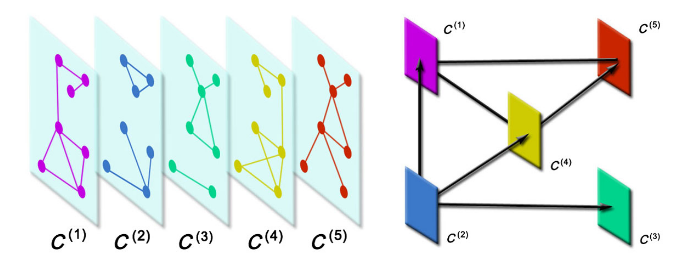
\includegraphics[width=\textwidth]{figures/multilayer_network}
	\caption{A schematic representation of a multilayer complex network. Here, $C^{(n)}$ is the $n$th layer of the network. The right hand figure shows how the layers connect to each other, forming a network of networks. This network would be represented as a four-dimensional tensor with each entry $a^{\alpha\beta}_{ij}$ corresponding to the strength of link form node $i$ in layer $\alpha$ to node $j$ in layer $\beta$. Figure taken from \cite{de2013mathematical}.}
\end{figure} 

\section{Active Module Identification}

While community detection only considers only the structure of the network at hand, often nodes in network may be enriched with additional attributes that are not solely based upon the observed topology of the network. For example, people in a social network may be annotated with preferences such as hobbies and interests and we would expect two people with the same interests to still somehow be similar, even if we do not observe a direct link between them in the network. Within the context of computational biology, this is perhaps even more relevant, due to the vast quantity and variety of data now available to us, and the successes of integrative models in the past. Integrative models get their name from the principle of integrating observed data (say, gene expression) with prior knowledge (often in the form of a known protein interaction network and/or previously curated functional annotations). \cite{mitra2013integrative} offers a summary of many the integrative approaches popular in the literature.

One of the most successful integrative approach is the identification of so-called `active modules'. It is a relatively recent trend within the interdisciplinary fields of network science and translational medicine and aims to augment known physical interactions with observed expression levels to identify connected sub-graphs (called sub-networks for the remainder of this proposal) that are maximally differently expressed. Ideker et al. was the first to formalise this problem in 2002 (\cite{ideker2002discovering}). Given a known PPI network $G$ and a matrix of gene expression levels with their corresponding p-values $P$, we compute a z-score for each gene $i$ in the network as:
\begin{align}
z_i = \Phi^{-1}(1 - p_i)
\end{align}
and then score identified sub-networks $A$ in an aggregated manner with 
\begin{align}
z_A = \frac{1}{\sqrt{k}}\sum_{i\in A}z_i
\label{ideker}
\end{align}
where a high $z_A$ represents a biologically active sub-network. Here, $\Phi^{-1}$ is the inverse normal CDF. While the problem is related to community detection -- the sub graphs must be connected -- but biologically relevant modules often do not align with communities based solely on network topology.

Computing an exact solution is NP-hard (\cite{ideker2002discovering}), so the authors employ a heuristic search based on simulated annealing to search for the maximally scoring sub-graph in the network. Genetic algorithms (GAs) (\cite{Klammer2010}), greedy methods (\cite{nacu2007gene}) and propagation of flow from cancer genes have since been used (\cite{vandin2011algorithms}). More recent work has employed a memetic algorithm to ensure connectedness (\cite{li2017active}); a multi-objective optimisation process to control the trade off between biological activity and functional enrichment of the detected modules (\cite{chen2017prior}); and a cooperative co-evolutionary approach (\cite{he2016cooperative}). Interestingly, despite the NP-hardness of the problem, \cite{dittrich2008identifying} showed that by transforming the above problem into the well known Prize Collecting Stein Tree (PCST) problem, exact solutions can be obtained in reasonable computational time with integer programming.

\begin{figure}
	\centering
	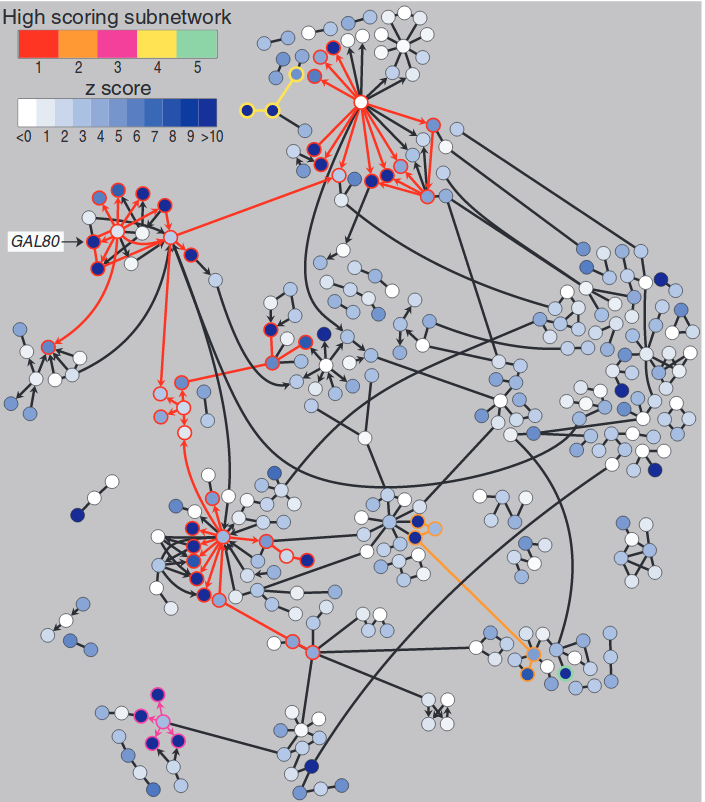
\includegraphics[width=\textwidth]{figures/ideker}
	\caption[Identified active modules in GAL80 knowckout experiment]{Top five active modules identified by a simulated annealing approach in \cite{ideker2002discovering}. Nodes in this network represent genes, undirected edges signify that the proteins encoded by these genes physically interact and a directed edge represents transcription influence. Nodes are colours by the likelihood of their observed expression change in a GAL80 knockout experiment. The subnetworks identified represent the most 'biologically active' modules in the network. Figure taken from \cite{ideker2002discovering}.}
\end{figure}


\section{Network Embedding}

Several models in the literature assume the existence of an underlying metric space that controls the topology of the network. They suppose that entities that are closer together in this space are more `similar' and have a higher probability of being connected. These models aim to infer the geometry of these spaces and the positions of nodes within the space, such that the probability of reconstructing the observed network is maximised, for purposed of better understanding of the system and visualisation. This is the so-called network embedding, and is the cornerstone of the field of \textit{network geometry}. 

Network embedding is closely related to the field of manifold learning. Indeed, many classical non-linear manifold learning techniques, such as Isomap (\cite{tenenbaum2000global}) and Laplacian Eigenmaps (\cite{belkin2002laplacian}), must first construct nearest neighbour graphs based on dissimilarities between samples before dimensionality reduction takes place. Many of these techniques are directly applicable to embedding of complex networks by simply omitting the graph construction step.

An interesting and popular embedding paradigm in the literature comes from natural language processing. In particular, the Skipgram model and the Word2Vec algorithm that aims to vectorise words and phrases in a semantic space such that similar words are mapped close together (\cite{mikolov2013distributed,mikolov2013efficient}). The principle idea is, given a corpus of words and a particular sentence, generate a `context' for each input word with the aim of maximising the likelihood of observing context words in the embedding space, given the input word. Similarities are measures by dot products and accordingly, observation probabilities are computed using a multilayer perception with a linear hidden layer and softmax output. Through the use of sub-sampling and negative sampling (replacing softmax with sigmoid), training can be made very efficient and the resulting embeddings can be obtained from the activation of the hidden units. This idea naturally extends to networks, where sentences are replaced by `neighbourhood graphs' generated from random walks. Furthermore, the shallow architecture of the Skipgram model has been replaced with multiple non-linear layers to learn the highly non-linear relationships between nodes (\cite{perozzi2014deepwalk,tang2015line}). By introducing additional parameters into the random walk to control a breadth vs. depth first neighbourhood search, \cite{grover2016node2vec} were able to identify neighbourhoods of nodes with high \textit{homophily} and high structural similarity. 

\subsection{Embedding to a Hyperbolic Metric Space}

An emerging popular belief in the literature is that the underlying metric space of most complex networks is in fact hyperbolic. Nodes in real world networks often form a \textit{taxonomy}, where nodes are grouped hierarchically into groups in an approximate tree structure. Hyperbolic spaces can be viewed as continuous representations of this tree structure and so models that embed networks into hyperbolic space have proven to be increasingly popular in the literature (\cite{krioukov2009curvature,krioukov2010hyperbolic}). In fact, this assumption has already had proven success in the task of greedy forwarding of information packets where nodes use only the hyperbolic coordinates of their neighbours to ensure packets reach their intended destination (\cite{papadopoulos2010greedy}). 

The most popular of all these models is the Popularity-Similarity (or PS) model (\cite{papadopoulos2011popularity}). This model extends the ``popularity is attractive'' aphorism of preferential attachment to include node similarity as a further dimension of attachment. Nodes like to connect to popular nodes but also similar ones. The PS model sustains that the clustering and hierarchy observed in real world networks is the result of this principle (\cite{alanis2016efficient}). This model has a simple interpretation in two dimensional hyperbolic space, where nodes are placed on a hyperbolic disk, with radial coordinates representing popularity and angular coordinates representing similarity. Then the hyperbolic distance between two nodes $\textbf{x}_1=(r_1, \theta_1)$ and $\textbf{x}_2=(r_2, \theta_2)$, given by  the hyperbolic law of cosines:
\begin{align}
d(\textbf{x}_1, \textbf{x}_2) &= \text{arccosh}(\cosh(r1)\cosh(r2) - \sinh(r1)\sinh(r2)\cos(\Delta\theta) \\
\Delta\theta &= \pi - | \pi - | \theta_1 - \theta_2 | |
\end{align}
controls their connection probabilities. Nodes with short hyperbolic distances show a higher probability of being connected.

Maximum likelihood (ML) was used in \cite{papadopoulos2011popularity} to search the space of all PS models with similar structural properties as the observed network, to find the one that fit it best. This was extended by the authors in \cite{papadopoulos2015network,papadopoulos2015networkgeo}. Due to the computationally demanding task of maximum likelihood estimation, often heuristic methods are used. For example, \cite{alanis2016efficient} used Laplacian Eigenmaps to efficiently estimate the angular coordinates of nodes in the PS model. The authors then combined both approaches to leverage the performance of ML estimation against the efficiency of heuristic search with a user controlled parameter in \cite{alanis2016manifold}. Additionally, \cite{thomas2016machine} propose the use of classical manifold learning techniques in the PS model setting with a framework that they call \textit{coalescent embedding}.

\begin{figure}
	\centering
	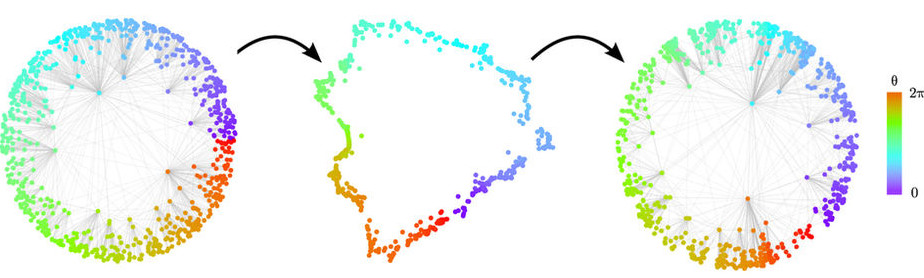
\includegraphics[width=\textwidth]{figures/LABNE}
	\caption[A hyperbolic network embedding algorithm in action]{An artificial complex network embedded onto the two dimensional hyperbolic disk. (a) an artificial network generated according to the PS model. (b) the LABNE algorithm in progress to determine each nodes radial coordinates according to the graph Laplacian. (c) determining radial coordinated by popularity (node degree). Figure taken from \cite{alanis2016efficient}.}
\end{figure}

\subsection{Embedding with Node Attributes and Dynamics}
Little work has been done to embed networks, accounting for both topology and node attributes, however recent years has shown it to become more prolific. \cite{gibert2012graph} embed into a vector space based on the statistics of attributes and pairs of attributes, \cite{li2017attributed} draw from the well known fields of manifold learning and multi-view learning to align the projections based on topology and attributes and \cite{liao2017attributed} use deep learning. In \cite{niepert2016learning}, the authors generalised convolutional neural networks from regular pixel lattices to arbitrary graphs. It is worth noting that by transforming an unweighted graph into a so-called `flow graph' (\cite{ISI:000293452500017}) by weighting links by node expression, many embedding techniques that are applicable to weighted graphs can be applied to unweighted graphs with node attributes. However, it is not clear how to do this if the graphs are already weighted, or nodes are annotated with discrete or multiple attributes.




\chapter{Proposed Work}

\section{Research Questions}
After a thorough literature review, the following research questions have been identified as the focus of the upcoming PhD:

\begin{enumerate}
	\item Can a multi-layer network model be constructed such that the hyperbolic metric space that underpins complex network formation be uncovered for multi-layer networks?
	\item What interpretable information, such as disease modules or functional predictions, can be extracted from such a model?
	\item My constructing data-driven models, can we predict protein abundance and phosphorylation?
\end{enumerate}

\section{Network Model Construction}
When constructing multilayer network models, the main challenge is the weighting of inter-layer links. Intra-layer links (such as protein-protein or metabolite-reaction links) are simple and constructed directly from the data. For example, we will place a link between proteins that physically interact or a link between a metabolite and a reaction if that metabolite is involved in that reaction, either as a \textit{substrate} or \textit{product}. Inter-layer links are placed between entities if they are related -- for example, a protein is part of a metabolite or is associated with a particular phenotype. 

\section{Network Embedding to Hyperbolic Metric Space}
Network embedding can be considered a preprocessing step for knowledge extraction from biological data. Knowledge such as disease module identification, for example. Embedding allows for the transformation of problems: from module to detection to clustering. But, selecting a metric space and embedding method is a very non-trivial problem. 

The recent trend towards models that support an underlying hyperbolic metric space is very appealing, as results are extremely positive, and the space is a generalisation of the hierarchical structure that we know actually exists in complex networks. However, there are a number of questions as yet unanswered that this work shall focus on. Firstly, how to embed networks with node attributes into hyperbolic space, such that active modules can be identifies as clusters. While single continuous node attributes can be combined with into the topology of an unweighted graph via construction of flow graphs (\cite{ISI:000293452500017}), some of the current hyperbolic embedding methods (for examples LABNE \cite{alanis2016efficient}) is unsuitable for weighted graphs. Furthermore, flow graphs cannot be used if there is more than one node attribute. Another challenge is embedding of multilayer networks.

This work will first attempt to tackle both of these problems for hyperbolic network embedding with the application of multi-view learning techniques. We will consider each layer as a separate view and align the separate embeddings onto the same space using, for example, kernel canonical correlation analysis (KCCA) (\cite{hardoon2004canonical}). In the case of networks with node attributes, we shall first construct an `attribute network' by connecting nodes with similar attributes, for example with KNN. Another technique that shall be adapted for the hyperbolic space is the recently proposed extension of convolutional neural networks to arbitrary graphs (\cite{niepert2016learning}). Additional ideas for future work include extending the currently used 2D hyperbolic plane to three dimensions to allow for simultaneous embedding of all layers. However, very little thought has been put into this currently.

\section{Module Identification and Knowledge Extraction}
The identification of modules has proven to be an important step in extracting knowledge from a complex network. It is clear from the literature that topological modules (communities) rarely align with complete functional modules, such as pathways (\cite{he2016cooperative}). Because of this, the addition of prior knowledge is essential to guide the module search to look beyond topology alone. Similarly, the identification of active modules must be guided by both node attributes (gene expressions) and network topology (identified sub-networks must be connected) (\cite{ideker2002discovering}). Furthermore, modules in biological networks have been shown to have a highly hierarchical structure -- where large modules of more general function are composed of many smaller ones that perform more specific tasks. As such, any model for meaningful biological module recovery must take hierarchy into account. Also, biological systems are dynamic -- in that their activity, and maybe even topology changes over time -- and composed of many types of entities and interactions. Because of this, network models must be scalable from single to multiple layers in tractable time. Finally, due to experimental error and measurement difficulties often data is incomplete and so any model must be robust enough to handle this. All of these factors combined make the problem of identifying the modular structure of biological systems a complex optimisation and combinatorial problem. This work intends to overcome some of the weaknesses of other techniques -- such as poor scalability or user-defined parameters to control the number of modules or module scale -- by developing models that allow for the extraction of modules in a more data-driven way.

The first such model will use the topology preserving property of the self-organising map to construct a map of communities based on an observed network. The model will use the Growing Hierarchical Self-Organising Map (GHSOM) (\cite{dittenbach2000growing}) to grow maps organically with no need to specify map size a priori. Furthermore, neurons in the map may be selected for expansion, resulting in new maps of higher granularity for those data points. This results in a set of maps with hierarchical structure that reflects the underlying hierarchical community structure of the data.

This model has a number of drawbacks, in that it is solely topology based, and requires some network embedding to a Euclidean (or perhaps hyperbolic) space or adaption of the algorithm to work directly on graphs, as in \cite{yamakawa2006self}. The map structure may also impose too strong an emphasis on module connection and so the Growing Hierarchical Neural Gas (\cite{palomo2016growing}) may be a more suitable choice, as it only connections between neurons are allowed also form in a data-driven way. It is also unclear how to scale this module to multiple layers without utilising some multi-view learning techniques to align the embeddings of the layers into the chosen space. Also, despite the appealing nature of not needing to know the number of modules or structure a priori, GHSOM is controlled by a number of parameters that can be difficult to tune.

Future work will attempt to generalise heuristic algorithms for active module identification to networks with many layers, such that the identified modules contain nodes from multiple layers. In the context of dynamical data, this will identify modules that are conserved across time points. Existing algorithms for multi-scale community detection (\cite{mucha2010community,ashourvan2017multi}) could be combined with heuristics to guide a search to include node scores as well as topology. 

\section{Protein Abundance and Phosphorylation Level Prediction}
Protein function almost always determines the biological function of a cell. As a result, proteomics (the study of proteins) is perhaps the most well studied area of computational biology. However, there are a number of challenges that face the proteomics research community today. Firstly, protein datasets are often incomplete, due to experimental errors and other challenges. As such, an method to effectively impute missing values would enable the community to access data that would otherwise be ignored in analyses. Furthermore, protein data is expensive to generate and not as readily available to the scientific community as Copy-Number Alterations (CNA) and mRNA data. It is well known that mRNA is used to transfer information to proteins, however it has been shown that RNA expression alone is weakly predictive of protein levels (\cite{vogel2012insights}). We would like to augment this analyses with the integration of CNA profiles -- which have been shown to affect protein abundances (\cite{zhang2016integrated}) -- for more accurate protein abundance prediction. Finally, by further integration of known proteomics profiles, we would like to predict the phosphorylation levels of proteins, as this has been shown to be one of the key so-called Post-translational Modifications (PTMs) that affect protein, and therefore cell, function. These challenges form the basis for the NCI-CPTAC DREAM Proteogenomics Challenge that this author, along with a distinguished team of researchers, shall participate in. 

Tackling the imputation challenge shall begin by performing a servery and comparison against ground truth of many common imputation techniques found in the literature. For example, sample means, matrix factorization, spectral regularization (\cite{mazumder2010spectral}), Multiple Imputation by Chained Equations (MICE), and an autoencoder with an adapted objective as in \cite{beaulieu2016missing}. The best algorithm shall be adapted to give improved performance.

Prediction of protein abundance and phosphorylation levels shall be tacked in a three stage way. First, by the application of simple machine learning techniques, such as regression models. Then, by constructing network models. Finally, by augmenting our models with the inclusion of domain knowledge than can be extracted from the given data, such as ribosome number and binding site information, provided by an expert in the field. 

\begin{figure}
	\centering
	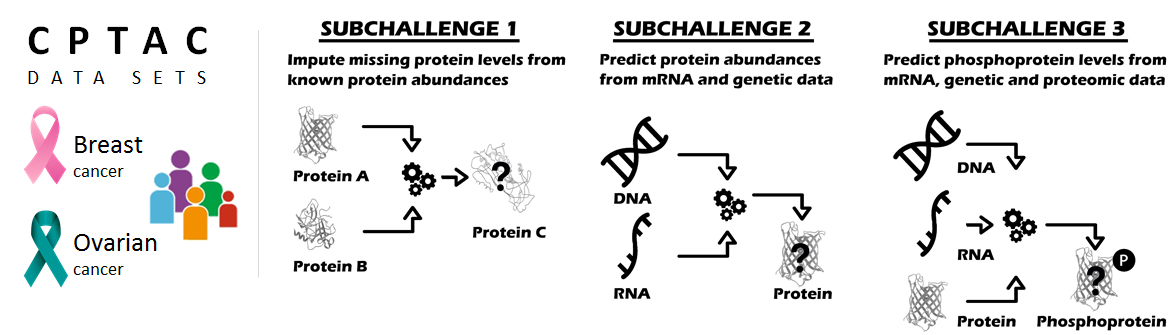
\includegraphics[width=\textwidth]{figures/DREAM}
	\caption[NCI-CPTAC DREAM Proteogenomics Challenge Sub-challenges]{Schematic representation of the three sub-challenges ion the NCI-CPTAC DREAM Proteogenomics Challenge. Sub-challenge 1: impute protein levels. Sub-challenge 2: predict protein abundances. Sub-challenge 3: predict phosphoprotein levels.}
\end{figure}



%\chapter{Preliminary Results}
%
%SOM paper -- results in question to be honest
%
%figures here


\chapter{Work Plan}

Table \cref{timeline} below details a detailed plan of the next year of work. The plan becomes much more general after than, as following work depends greatly upon the success of my early work and any new developments in the field. A Gantt chart generated from this table is available in the appendix.

\begin{table}[htb]
	\centering
	\csvautobooktabular{gantt.csv}
	\caption{Timeline of proposed PhD. Gantt chart can be found in the appendix.}
	\label{timeline}
\end{table}




\chapter{Implications of Research}

The main purpose of the work proposed here is to provide that can better make sense of all the data that is produced by bioscientists every day. It will generate knowledge from data through the means of extracting useful and interpretable features from complex network models that allow for the automatic generation of predictions or further study by domain experts. This will be achieved through novel network construction, embedding and feature extraction methods. 

Hyperbolic network embedding has been shown to help uncover and understand how complex networks are formed (\cite{krioukov2010hyperbolic}). Furthermore, it has successfully predicted missing links in networks (\cite{alanis2016efficient}), which is particularly relevant to biosciences as testing for physical protein interactions is an expensive procedure that benefits from predictive models guiding the experimentation. Generalising these models to multiple levels may potentially allow for link prediction across different entities. For example, proteins and Gene Ontology terms that they have not yet been assigned to. Furthermore, multi-level hyperbolic embedding may be able to uncover a hierarchical structure that considers all entities in the system, rather than the structure of the entities amongst amongst themselves.

This will further be enhanced by more sophisticated module detection schemes. Schemes that are able to successfully harness to the topology of the network to detect subnetworks that not only show high biological activity but also high functional cohesion, while preserving the known hierarchical organisation of biological modules, in a data-driven way with few parameters to tune. This will allow for a deeper and more comprehensive understanding of how biological systems form and what role each member of the system plays. 

We know that protein abundance is often indicative of cellular function, and yet proteomic profiling data from mass spectrometry based experiments often contain a large number of missing values due to the dynamic nature of the mass spectrometry instruments. This data is valuable and we would not wish to discard it out of hand. RNA/DNA is much cheaper to generate and more widely available than proteomic data, but RNA alone is only weakly predictive (\cite{vogel2012insights}). Development of a novel imputation method, based on machine learning and network science techniques would allow bioscientists to harness data to its full capacity with high confidence. And new protein abundance and phosphorylation level prediction techniques will result in improved biomarker development and avoid expensive enrichment testing. 

%----------------------------------------------------------------------------------------
%	THESIS CONTENT - APPENDICES
%----------------------------------------------------------------------------------------


%----------------------------------------------------------------------------------------
%	BIBLIOGRAPHY
%----------------------------------------------------------------------------------------

\printbibliography[heading=bibintoc]

%----------------------------------------------------------------------------------------


\appendix % Cue to tell LaTeX that the following "chapters" are Appendices

% Include the appendices of the thesis as separate files from the Appendices folder
% Uncomment the lines as you write the Appendices
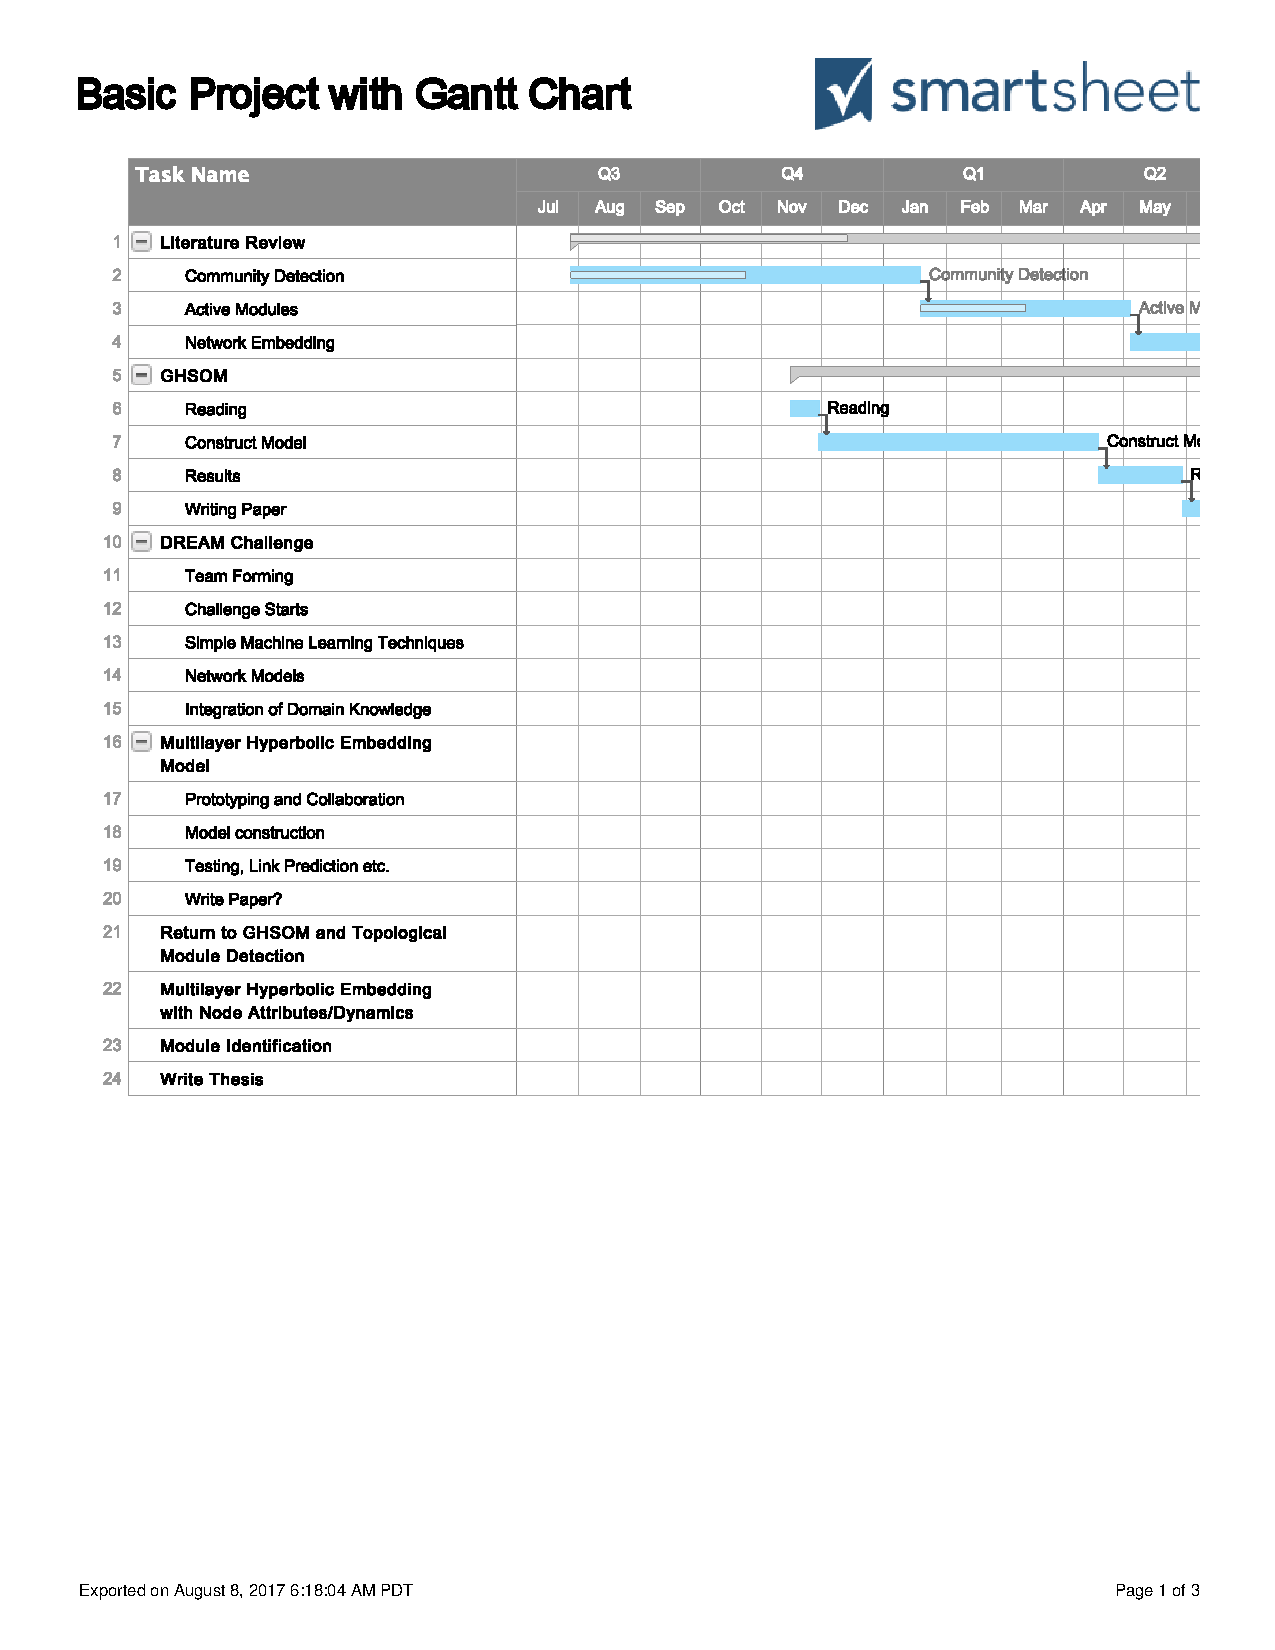
\includepdf[pages=-]{gantt}

%\include{Appendices/AppendixA}
%\include{Appendices/AppendixB}
%\include{Appendices/AppendixC}

\end{document}  
